\section{System test}
After the assembling of the PCB and testing the components behave like the expectation, the complete system test is performed. For the tests the PV simulator \textit{E4360} from Keysight Technologies \cite{PV_simulator} is used to simulate the PV panel \textit{STP300S-24/Vd} from Suntech Power \cite{PV_panel}. At first the converter is subjected the open loop test. The reason of this test is to compare the measured voltages and current ripples with the values from the ideal open loop simulation in appendix \ref{app:OL_ripple}. The second test includes the thermal test. For this test the converter is performed for a longer time to identify which parts of the PCB will be overheated. The last test is about validating the P\&O algorithm, if it behaves like in the simulation from section \ref{MPPTSimulation}.

\subsection{Open loop test}

The open loop test is carried out to measure the ripples in the inductor current, the input voltage and the output voltage of the converter. The test conditions were explained in section \ref{sec:componentsizing} and the graphs showing the experimental results are shown in appendix \ref{app:OL_ripple}.

The measured current ripple in the inductor is calculated from figure \ref{Openlooptestinductor} and shown in equation \ref{eq:inductor_ripple}. The minimum current is $I_{min} = 2.7A$ and the maximum current is $I_{max} = 2.98A$. The mean value for the inductor current is $\widebar{I_L}= 2.84$. 

\begin{equation} \label{eq:inductor_rippleexpirment}
\Delta I_L = \frac{I_{max}-I_{min}}{\widebar{I_L}} \cdot 100 = \frac{2.98A-2.7A}{2.84A} \cdot 100 = 9.86\%
\end{equation}

The result obtained for the output voltage ripple is shown in figure \ref{Openlooptestoutputtcapacitor}. The ripple percentage is calculated in equation \ref{eq:output_voltage_rippleexperiment} using the values obtained from the graph. 

\begin{equation} \label{eq:output_voltage_rippleexperiment}
\Delta V_{out} = \frac{V_{out,max}-V_{out,min}}{\widebar{V_{out}}} \cdot 100 = \frac{23.9082V - 23.895V }{23.9V} \cdot 100 = 0.055\%
\end{equation}

Finally, the measured input voltage ripple is shown in figure \ref{Openlooptestinputcapacitor}. It is observed from the figure that the signal is too noisy and it is not possible to identify the real voltage ripple. This is because the input voltage ripple was defined to be lower than 0.1\% and, as the input capacitor has a high capacitance, the measured ripple is neglected. \todo{check this and if it's necessary explain it better. Stef}

\subsection{Thermal test}

For this test, the converter is supplied for 10 minutes (or 600 seconds) a constant input voltage 36.9 V and input current 7 A. Tthe converter is performing in buck mode with the fix duty cycles D1 = 0.8 and D2 = 0 in this test. The temperature of the components coil, heat sink and security diode are measured during the test because they are the critical components. Figure \ref{Testthermal} shows that the diode is produced the most amount of heat.\todo {thats not true. This is only a random sentence.}

\begin{figure}[H]
	\begin{center}
		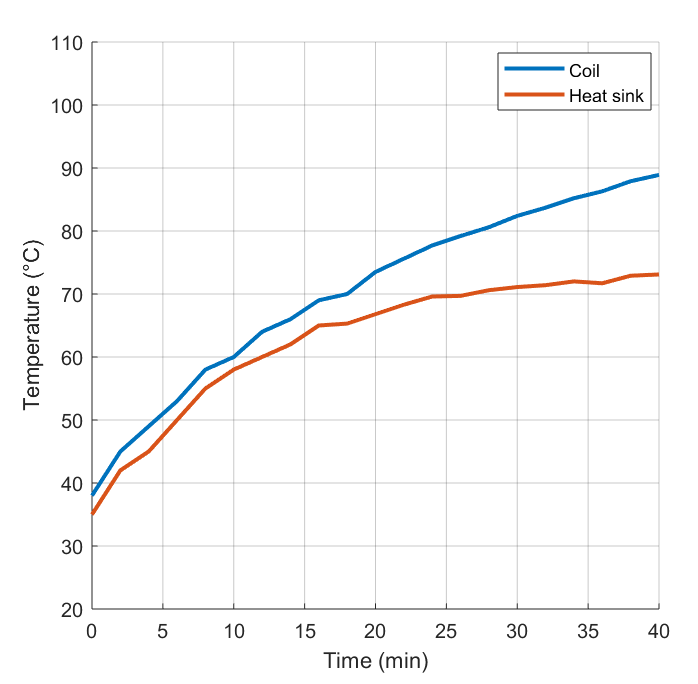
\includegraphics[width=0.65\textwidth]{../Pictures/P1/Test/Thermal_test_with_heat_sink}
		\caption{Thermal test.}
		\label{Testthermal}
	\end{center}	
\end{figure}

\subsection{MPPT test}
The section MPPT test is divided in two parts. One part is that the converter is working with the P\&O to find the MPP .The other part is that during the converter with the P\&O MPPT algorithm is in operation the ambient conditions will change in temperature or irradiance. The tests are compared with the result from section \ref{MPPTSimulation}. The PV-panel voltage and current is in all figures the input voltage and current from the converter.

In the first part the converter is operated one time in buck and boost mode. For both modes the ambient condition is for the irradiance 1000 $W /m^2$ and for the temperature 25 $\decC$ (as STC ). If the converter is performed in the buck mode, the load is 3 $\Omega$ at the output from the converter. For the boost mode the load is 27 $\Omega$ at the output.

The figure \ref{MPPTtestbuckmode1} shows that the converter is finding the MPP in buck mode. The left graph represents the input and the current of the converter. At first the input voltage reached the open circuit voltage as in the simulation.  After 10 seconds the P\&O algorithm reaches the MPP. In steady state the converter extracts 294 W from the PV-panel which can be seen in the right graph in figure \ref{MPPTtestbuckmode1}.This value is smaller than the value from the datasheet \cite{PV_panel}
\todo{for the future: compare with the values from simulation with  experiment in one graph but consider that the simulation should run for 40 seconds to plot both in one graph}

\begin{figure}[H]
	\begin{center}
		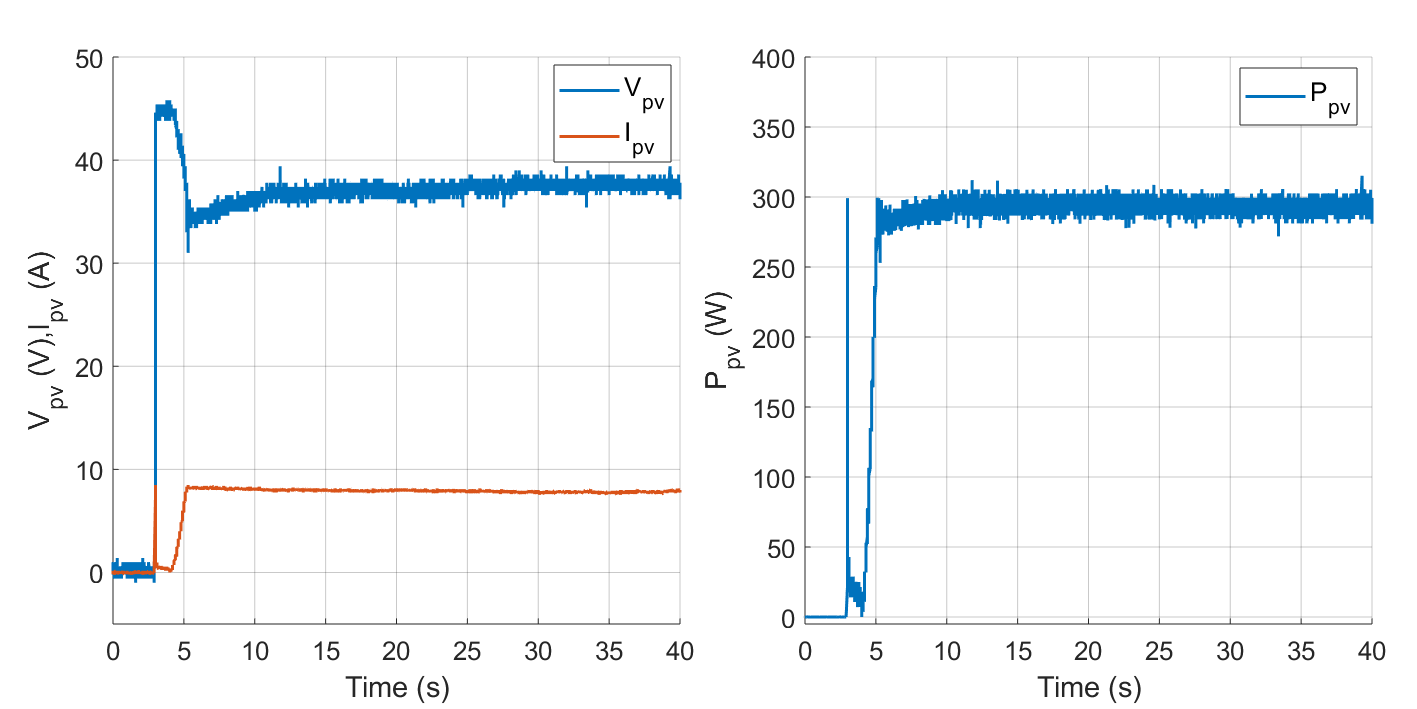
\includegraphics[width=1\textwidth]{../Pictures/P1/Test/Buck_mode_MPPT_Vin_Iin_Pin}
		\caption{MPPT test: converter extracts voltage, current and power from the PV-panel in buck mode.}
		\label{MPPTtestbuckmode1}
	\end{center}	
\end{figure}

In the left graph in figure \ref{MPPTtestbuckmode2} is observed the relationship between input and output voltage from the converter. So the converter decreases the output voltage in steady state.\todo{here should stand the equatio for the duty cycle}
 
\begin{figure}[H]
	\begin{center}
		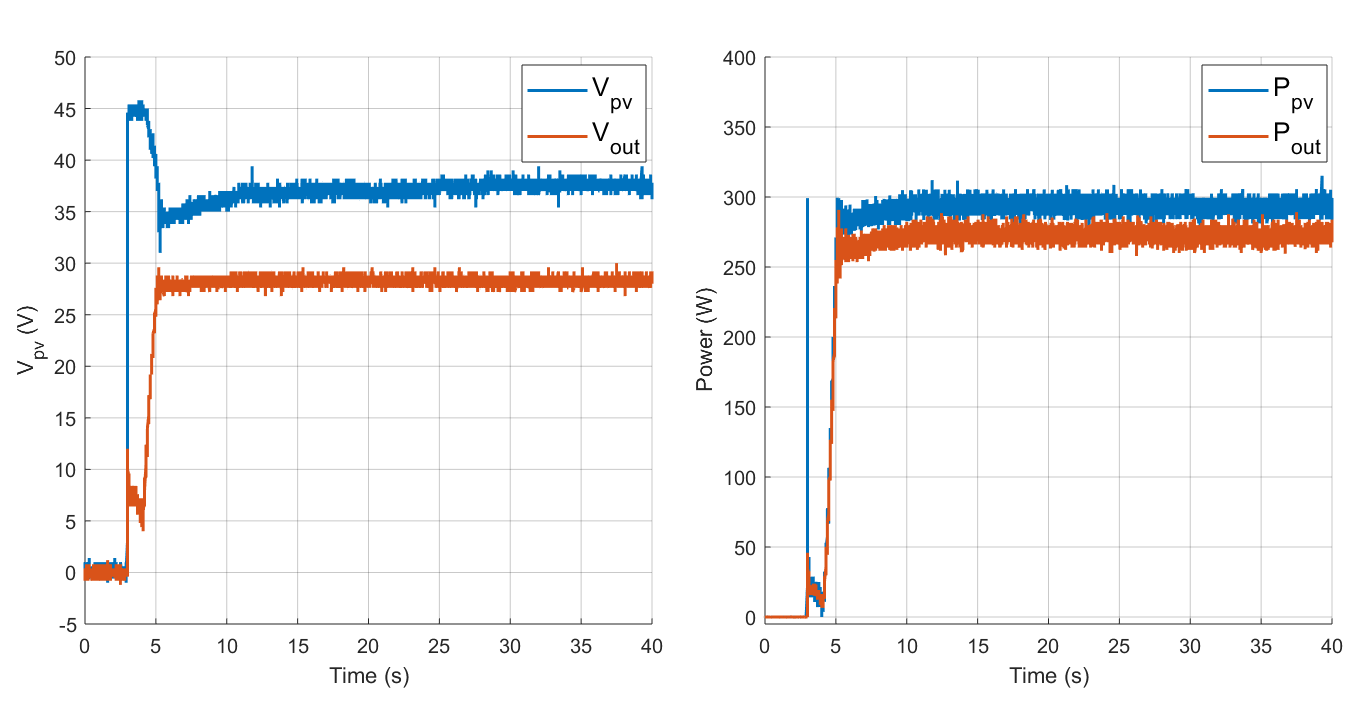
\includegraphics[width=1\textwidth]{../Pictures/P1/Test/Buck_mode_MPPT_Vin_Vout_Pin_Pout}
		\caption{MPPT test: converter behavior in buck mode.}
		\label{MPPTtestbuckmode2}
	\end{center}	
\end{figure}

\todo{maybe for the figure MPPTtestbuckmode2 the figure with the duty cycle}


boost mode

\begin{figure}[H]
	\begin{center}
		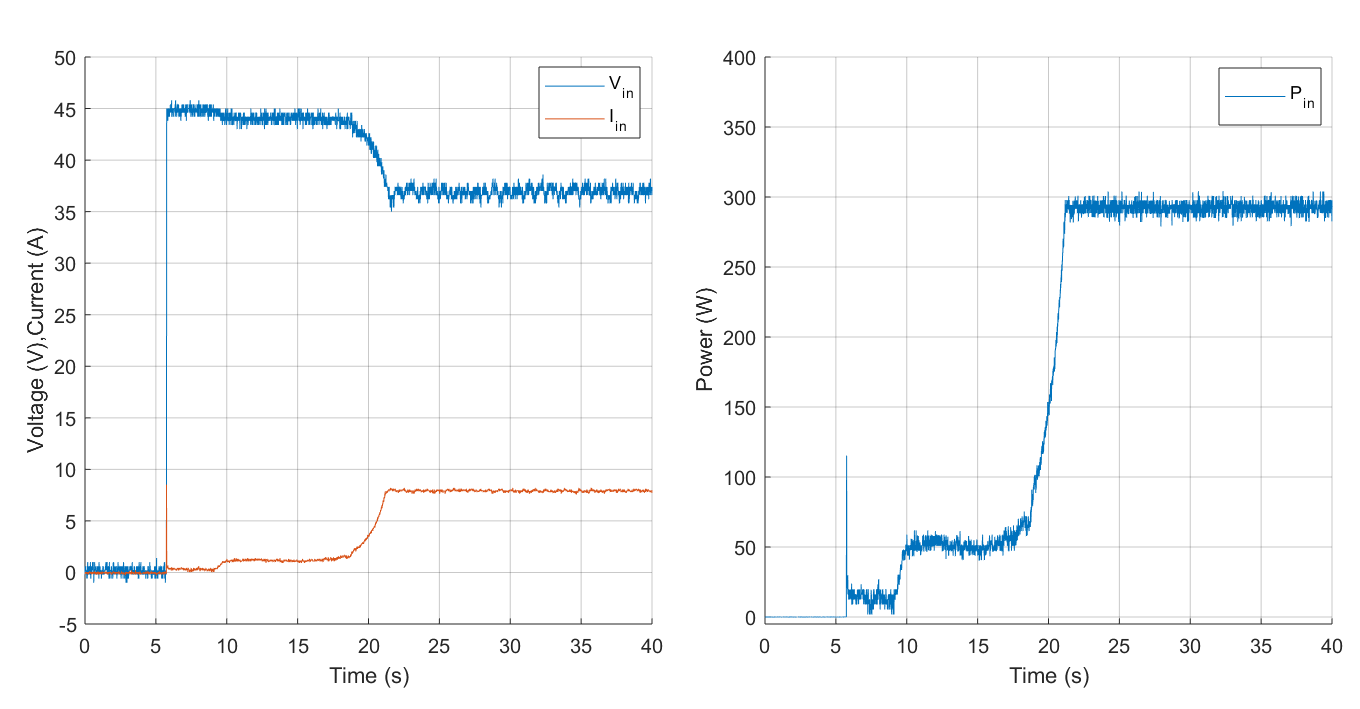
\includegraphics[width=1\textwidth]{../Pictures/P1/Test/Boost_mode_MPPT_Vin_Iin_Pin}
		\caption{MPPT test: converter extracts voltage, current and power from the PV-panel in boost mode. picture not right}
		\label{MPPTtestboostmode1}
	\end{center}	
\end{figure}

\begin{figure}[H]
	\begin{center}
		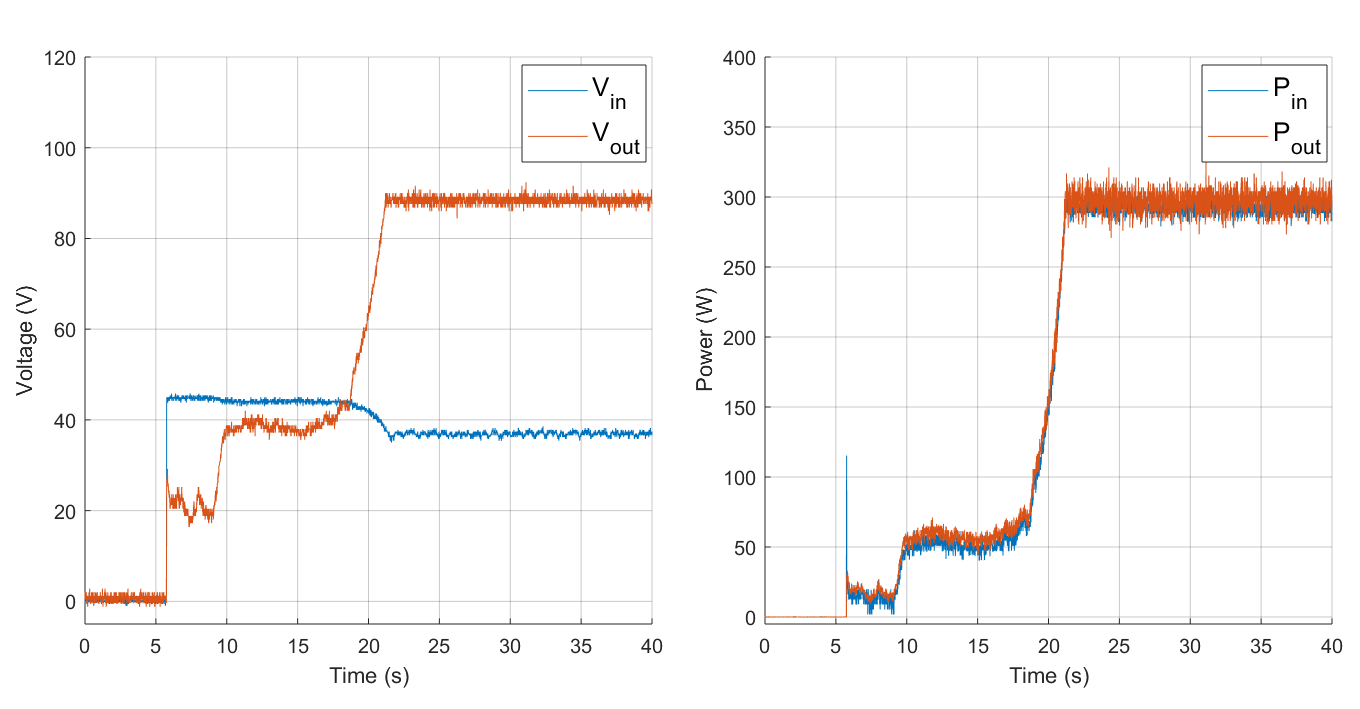
\includegraphics[width=1\textwidth]{../Pictures/P1/Test/Boost_mode_MPPT_Vin_Vout_Iin_Pin_Pout}
		\caption{MPPT test: converter behavior in boost mode.}
		\label{MPPTtestboostmode2}
	\end{center}	
\end{figure}




